\documentclass[a4,abstract=on]{scrartcl}

\usepackage[utf8]{inputenc}
\usepackage[T1]{fontenc}
\usepackage{placeins}
\usepackage{graphicx}
\usepackage[hypcap]{caption}
\usepackage{algorithm}
\usepackage[noend]{algpseudocode}
\usepackage[hidelinks]{hyperref}
\usepackage[nochapters]{classicthesis} % nochapters, wenn du section als oberste ebene nimmst
\usepackage{array}
\PassOptionsToPackage{big}{titlesec}

\floatname{algorithm}{Algorithmus}
% Mathe
\usepackage{amsmath}
\usepackage{amssymb}


% Verlinkungen
\usepackage[ngerman]{varioref} % Siehe http://en.wikibooks.org/wiki/LaTeX/Labels_and_Cross-referencing#The_varioref_package
%\usepackage[hidelinks]{hyperref}

% Spracheinstellungen sowie Umlaute etc.
\usepackage[ngerman]{babel}
\usepackage{ngerman}

% Bilder
\usepackage{graphicx}

% Tabellen-Abstand
\renewcommand{\arraystretch}{1.5}

% Quellcode
\usepackage{listings}
\lstset{%
	breaklines=true,
	frame=single,
	keepspaces=true,
	numbers=left,
	numbersep=5pt,
	tabsize=2
}

% Literatur
\usepackage{bibgerm}
\usepackage{natbib}

% Lässt sections immer auf der ungeraden (rechten) Seite anfangen.
    \newcommand*\stdsection{}
    \let\stdsection\section
    \renewcommand*\section{%
    \clearpage\ifodd\value{page}\else\mbox{}\clearpage\fi
    \stdsection}

% neuer Typ von Tabellenspalte (so wie c, l, etc.). Ist zentriert mit fester Breite.
\newcolumntype{C}[1]{>{\centering\let\newline\\\arraybackslash\hspace{0pt}}m{#1}}

% \usepackage{setspace}
% \onehalfspacing
\title{Untersuchung verschiedener Kodierungen von speziellen Cardinality Constraints für SAT}
\date{~}

\begin{document}
	\maketitle
\thispagestyle{empty}
\begin{center}
\begin{Large}
Bachelorarbeit\\Universität Bremen\\Fachbereich $3$\\
~\\~\\
\textbf{Jil Tietjen}\\<jiltietj@informatik.uni-bremen.de>\\
~\\~\\
Erstgutachter: Prof. Dr. Rolf Drechsler\\
Zweitgutachter: Prof. Dr. Rüdiger Ehlers\\~\\
\mbox{Betreuung: Prof. Dr. Rolf Drechsler \&~Oliver Keszöcze}\\~\\~\\~\\~\\~\\~\\~\\
Bremen, $09$. Juni $2016$
\end{Large}
\end{center}
		
	\newpage
~\\
\textbf{Urheberrechtliche Erklärung}\\
Erklärung gem. § $10$ ($10$) Allgemeiner Teil der BPO vom $27$.$10$.$2010$
Hiermit versichere ich, dass ich meine Bachelorarbeit ohne fremde Hilfe angefertigt habe, und dass ich keine anderen als die von mir angegebenen Quellen und Hilfsmittel benutzt habe.\\
Alle Stellen, die wörtlich oder sinngemäß aus Veröffentlichungen entnommen sind, habe ich unter Angabe der Quellen als solche kenntlich gemacht.\\
Die Bachelorarbeit darf nach Abgabe nicht mehr verändert werden.\\
~\\~\\~\\
Bremen, den $09$.$06$.$2016$\\
~\\~\\~\\
Jil Tietjen
~\\~\\~\\~\\~\\~\\
Ich bin damit einverstanden, dass meine Abschlussarbeit im Universitätsarchiv für wissenschaftliche Zwecke von Dritten eingesehen werden darf.\\
~\\~\\~\\
Bremen, den $09$.$06$.$2016$\\
~\\~\\~\\
Jil Tietjen
\clearpage

	\tableofcontents
	\clearpage

\section{Einleitung}
\section{Grundlagen}
\subsection{SAT-Problem}
Das Satisfiability Problem (kurz: SAT) ist das Erfüllbarkeitsproblem der Aussagenlogik. Es ist NP-vollständig und lässt sich daher vermutlich nicht in polynomieller Zeit lösen. Die Eingabe ist eine aussagenlogische Formel F für die heraus gefunden werden soll, ob sie erfüllbar ist. Es wird also eine erfüllende Belegung der Variablen mit true oder false gesucht. Die Formel F liegt üblicherweise in Konjunktiver Normalform (KNF) vor. Sie ist in konjunktiver Normalform, wenn sie eine Konjunktion von Disjunktionen von Literalen ist.\\
\begin{itemize}
\item $F = \bigwedge_{i=1, \dots ,n} \bigvee_{j=1,\dots ,m_i}{l_{i,j}}$\\
\end{itemize}
Ein Literal ist dabei eine Formel der Form $x$ oder $\neg x$, wobei $x$ eine atomare Variable ist.\\
Eine SAT-Instanz wäre zum Beispiel $(\neg a) \wedge (b \vee \neg c \vee d) \wedge (a \vee \neg b)$  für die es folgende Lösung gibt: $a = \bot, b = \bot, c= \bot, d = \top$. Es muss eine Belegung gefunden werden, so dass jede Klausel true ist.
Eine Klausel ist eine endliche Menge von Literalen. Bei einer KNF-Formel wird die Klauselmenge M(F) wie folgt zugeordnet:\\
\begin{itemize}
\item $i$-te Disjunktion $\bigvee_{j=1,\dots ,m_i}{l_{i,j}}$ erzeugt Klausel $C_i = \{l_{i1}, \dots, l_{im_i}\}$
\item M(F) = $\{C_1, \dots, C_n\}$
\end{itemize}
\subsubsection{SAT-Solver}
%DPLL
\subsubsection{Cardinality Constraint}
\subsubsection{Tseitin-Transformation}
\subsection{Sorting Networks}
Sorting Networks ermöglichen das parallele Verarbeiten von Algorithmen. Hierbei werden die Eingangsvariablen sortiert, so dass am Ende die Eingangsvariablen, die mit true belegt sind, oben angeordnet sind und die Variablen, die mit false deklariert werden in der unteren Hälfte angeordnet sind. Dies ist möglich durch einzelne Comparators zwischen zwei verschiedenen Leitungen. Ein Comparator hat somit zwei Eingangsvariablen und zwei Ausgangsvariablen, wobei die Ausgangsvariablen so sortiert werden, dass ein Ausgang den Maximumwert darstellt und der andere Ausgang den Minimumwert. 

\section{Kodierungen}
In diesem Kapitel werden die unterschiedlichen Kodierungen beschrieben. Das Ziel ist es, dass die Cardinality Constraints über die Menge der Boolschen Variablen in eine Konjunktive Normalform (KNF) gebracht werden. %Innerhalb der KNF gibt es Einschränkungen, die verlangen, dass höchstens $r$ der Booleschen Variablen 1 sein können. Rein in die Grundlagen
Das Cardinalitiy Constraint ist genau dann erfüllt, wenn die aus der Kodierung resultierende Formel erfüllt ist. Ein einzelnes Cardinality Constraint ist immer erfüllbar. Erst eine Kombination mehrerer Cardinality Constraints kann zu einer unerfüllbaren Formel führen.

%Evaluation Alle Kodierungen werden anhand des Damen-Problems und anhand einer Tomography auf ihre Praxistauglichkeit überprüft.

	\subsection{naiver Ansatz}
Zur Verdeutlichung der Einflüsse der weiteren Kodierungen wird als Erstes der naive Ansatz erläutert. Für den Fall $r=1$ wird aus allen möglichen Paaren von Variablen $x_i$ und $x_j$ die Klausel $\neg x_i \vee \neg x_j$ gebildet. Das bedeutet, dass beispielsweise $\sum(x,y,z)\leq1$ zu $(\neg x \vee \neg y) \wedge (\neg x \vee \neg z) \wedge (\neg z \vee \neg y)$ wird.
Für beliebige $r$ gibt es nicht nur Paare von Variablen, sondern $(r+1)$-Tupel.

% Um alle Möglichkeiten auch bei einer großen Anzahl von Variablen zu erfassen, wird als Grundlage die Mengenlehre angewendet. Es werden Untermengen erstellt, die sich mit folgendem System aufbauen. Das erste Element in der Menge bleibt immer gleich und für das zweite Element wird immer das nächst grössere Element ausgewählt. Eine Menge besteht immer aus den Teilmengen des ersten Index des Arrays vereinigt mit dem Element aus dem zweiten Index, aus dem dritten Index und so weiter. Dies wird rekursiv so lange fortgeführt bis alle Teilmengen erstellt sind. Die gebildete KNF kann schließlich mit $r$ verglichen werden.\\
Durch den folgenden Beweis kann gezeigt werden, dass die naive Kodierung für $r=1$ korrekt ist. Zu zeigen ist, dass wenn ein Constraint $C(x_1, \dots, x_n) = \sum(x_1, \dots,x_n) \leq 1$ für eine beliebige vollständige Belegung $v(x_1, \dots ,x_n)$ erfüllt wird, dann wird auch die naive Kodierung von $C(x_1, \dots, x_n)$ erfüllt.\\
Es wird angenommen, dass $v(x_1, \dots ,x_n)$ das Constraint $C(x_1, \dots, x_n)$ erfüllt. Das heißt, dass es maximal eine Variable $x_i$ mit $v(x_i) = \top$ gibt. Für alle anderen Variablen $x_j$ mit $i \neq j$ gilt $v(x_j) = \bot$. Durch das Encoding gibt es in jeder Klausel genau $2$ negierte Literale, somit gibt es in jeder Klausel mindestens eine Variable mit dem Wert $\bot$. Daraus folgt, dass jede Klausel erfüllt ist. Somit ist auch die gesamte KNF erfüllt.\\
Außerdem ist zu zeigen, dass wenn das Constraint $C(x_1, \dots, x_n) = \sum(x_1, \dots,x_n) \leq 1$ für eine beliebige vollständige Belegung $v(x_1, \dots ,x_n)$ nicht erfüllt wird, dann wird auch die naive Kodierung von $C(x_1, \dots, x_n)$ nicht erfüllt.\\
Es wird angenommen, dass $v(x_1, \dots ,x_n)$ das Constraint $C(x_1, \dots, x_n)$ nicht erfüllt. Somit gibt es $x_i, x_j; i \neq j$ mit $v(x_i) = v(x_j) = \top$. Durch das naive Encoding gibt es eine Klausel $(\neg x_i \vee \neg x_j)$, die nicht erfüllt wird. Somit ist auch die gesamte KNF nicht erfüllt.


	\subsection{Kodierung nach Bailleux und Boufkhad}
Im Folgenden wird die Kodierung aus \cite[][]{bailleux} vorgetellt. Im weiteren Verlauf werden zusätzlich Formeln aus \cite[][]{knuth} hinzugezogen.
%Diese Kodierung ist, laut Bailleux, effizient mit Berücksichtigung der Unit Propagation, die in den meisten Sat-Solvern verwendet wird. Es werden O(n log (n)) Variablen und O($\text{n}^2$) Klauseln gefordert, die aus mindestens 3 Literalen bestehen. Bei dieser Kodierung ist das Besondere, dass es eine einstellige Darstellung von Integer-Variablen gibt, die nicht nur den Wert an sich repräsentieren, sondern auch einem Intervall zugeordnet werden kann. Zum Beispiel gilt die Variable c nur, wenn das Intervall der Variablen ($a + b$) c erfüllt. Dadurch erhält man eine KNF. Die Kodierung muss korrekt sein, wenn es eine wahre Zuordnung gibt die unter der Berücksichtigung der Constraints erfüllbar ist.

%n erklären in den Grundlagen
Bei dieser Kodierung soll ein binärer Baum aufgebaut werden. Aus dem binären Baum können anhand von Formeln Literale gebildet werden. Durch das Wegstreichen von trivialen Variablen bleiben am Ende einige Klauseln mit einem Literal übrig. Für diese Literale kann sehr schnell eine Belegung gefunden werden. Dies steigert die Effizienz der Kodierung.

Der Baum wird iterativ aufgebaut und beginnt mit einem Wurzelknoten, der mit $1$ betitelt wird. Des Weiteren gibt es $n-1$ interne Knoten, sowie $n$ Blätter, die von $n$ bis $2n-1$ beschriftet werden. Die Kinder von Knoten $k$  für $1 \leq k \textless n$, sind die Knoten $2k$ und $2k +1$.
Jedem Knoten wird eine Menge von Variablen zugeordnet. Dabei wird jedem Blatt eine Eingangsvariable und dem Wurzelknoten die Menge der Ausgangsvariablen zugeordnet. Nun wird die Kodierung so aufgebaut, dass die Variablen eines inneren Knotens die Summe der Variablen seiner Kindsknoten repräsentieren. Daraus ergibt sich ein Wurzelknoten, dessen Variablen mit $r$ verglichen werden können, da sie die Summe aller Eingangsvariablen repräsentieren.\\

Als nächster Schritt werden neue Hilfsvariablen der Form $\text{b}_j^k$ gebildet, für $1 \textless k \textless n$ und  $1 \leq j \leq t_k$. Dabei ist $t_k$ das Minimum von $r$ und der Anzahl der Blätter unter dem Knoten $k$. Bei $n=2$ und $r=2$ hat der Knoten $1$ zum Beispiel $2$ Blätter, daher ist $t_1=2$. Jedem inneren Knoten k wird die Menge der Variablen $\text{b}_j^k$ zugeordnet.\\
Mit den neuen Variablen können folgende Klauseln gebildet werden:\\
\textbf{1. Formel:}\\
$ \neg \text{b}_i^{2k} \vee \neg \text{b}_j^{2k+1} \vee \neg \text{b}_{i+j}^{k}$ \\
für $0\leq i \leq \text{t}_{2k}$, $0\leq j \leq \text{t}_{2k+1}$, $1\leq i+j \leq \text{t}_{k}+1$, $1\textless k \textless n$\\
\textbf{2. Formel:}\\
$ \neg \text{b}_i^2 \vee \neg \text{b}_j^3$ für $0\leq i \leq \text{t}_2$, $0\leq j \leq \text{t}_3$, $i+j = r+1$\\

Dabei wird $\text{t}_k$ zu $1$ und $\text{b}_1^k = \text{x}_{k-n+1}$ für $n \leq k \textless 2n$. Dadurch können aus den Hilfsvariablen die entsprechenden Literale gebildet werden, die die KNF bilden.
Aufgrund des Aufbaus der Formel können Variablen der Form $b_{r+1}^k$ nur positiv und Variablen der Form $\text{b}_0^k$ nur negativ vorkommen. Daher können diese Variablen gestrichen werden.

\subsubsection{Beispiel für die Kodierung}
Für das Beispiel ist $n=4$ und $r =1$. Der binäre Baum hat $4-1 = 3$ interne Knoten, sowie 4 Blätter, die beschriftet sind mit $4$ bis $2*4-1=7$. Die Kinder von Knoten $1$  für $1 \leq 1 \textless 4$, sind die Knoten $2$ und $2*1 +1=3$. Daraus ergibt sich der binäre Baum, der in Abbildung \ref{fig:baum} zu sehen ist.

\begin{figure}[H]
\centering
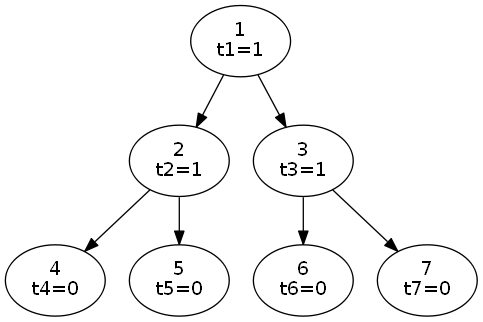
\includegraphics[width=9cm]{bailleux.png}
\caption{Binärer Baum nach Bailleux}
\label{fig:baum}
\end{figure}

Der Knoten $1$ hat die Blätter $4,5,6$ und $7$. Der Wert von $t_1$ ist daher $min(4,r) = min(4,1) = 1$. Die weiteren Variablen $\text{t}_2$ und $\text{t}_3$ sind auch jeweils $1$ und $\text{t}_4$ bis $\text{t}_7$ sind $1$, da $\text{t}_k$ zu $1$ wird, wegen $n \leq k \textless 2n$.

Dadurch ergeben sich für das Beispiel von $n=4$ folgende Variablen:\\
\textbf{Formel 1:}\\
$k=2$ oder $k=3$, weil $1 \textless k \textless n$.\\
$j=0$ oder $j=1$, weil $1 \leq j \leq \text{t}_k$ und $\text{t}_k = 1$.\\
$i=0$ oder $i=1$, weil $1\leq i+j \leq \text{t}_{k}+1$.\\
Somit ergeben sich für (i, j) die Möglichkeiten $(1,0)$, $(0,1)$ und $(1,1)$.\\
\textbf{k = 2:}\\
$\neg \text{b}_1^4 \vee \neg \text{b}_0^5 \vee \text{b}_1^2$\\
$\neg \text{b}_0^4 \vee \neg \text{b}_1^5 \vee \text{b}_1^2$\\
$\neg \text{b}_1^4 \vee \neg \text{b}_1^5 \vee \text{b}_2^2$\\
\textbf{k = 3:}\\
$\neg \text{b}_1^6 \vee \neg \text{b}_0^7 \vee \text{b}_1^3$\\
$\neg \text{b}_0^6 \vee \neg \text{b}_1^7 \vee \text{b}_1^3$\\
$\neg \text{b}_1^6 \vee \neg \text{b}_1^7 \vee \text{b}_2^3$\\

Da alle Variablen der Form $\neg \text{b}_0^k$ und $\text{b}_{r+1}^k$  gestrichen werden, bleiben nur noch diese Klauseln übrig:\\
\textbf{k = 2:}\\
$\neg \text{b}_1^4  \vee \text{b}_1^2$\\
$\neg \text{b}_1^5 \vee \text{b}_1^2$\\
$\neg \text{b}_1^4 \vee \neg \text{b}_1^5$\\
\textbf{k = 3:}\\
$\neg \text{b}_1^6 \vee \text{b}_1^3$\\
$\neg \text{b}_1^7 \vee \text{b}_1^3$\\
$\neg \text{b}_1^6 \vee \neg \text{b}_1^7 $\\

$b_1^k$ wird ersetzt durch $x_{k-n+1}$:\\
$ \neg \text{x}_1 \vee \text{b}_1^2$\\
$\neg \text{x}_2 \vee  \text{b}_1^2$\\
$\neg \text{x}_1 \vee \neg \text{x}_2$\\
$\neg \text{x}_3 \vee \text{b}_1^3$\\
$\neg \text{x}_4 \vee \text{b}_1^3$\\
$\neg \text{x}_3 \vee \neg \text{x}_4$\\

\textbf{Formel 2:}\\
$i=1$, weil $0\leq i \leq \text{t}_2$ für $\text{t}_2 = 1$.\\
$j=1$, weil $0\leq j \leq \text{t}_3$ für $\text{t}_3=1$.\\
Somit ergibt sich für (i, j) die Möglichkeit $(1,1)$, so dass $i+j = r+1$ gilt.\\
$\neg \text{b}_1^2 \vee \neg \text{b}_1^3$\\

Es können keine Variablen gestrichen werden.\\

Die vollständige KNF sieht folgendermaßen aus:\\
($ \neg \text{x}_1 \vee \text{b}_1^2$) $\wedge$ ($\neg \text{x}_2 \vee \text{b}_1^2$) $\wedge$ ($\neg \text{x}_1 \vee \neg \text{x}_2$) $\wedge$ ($\neg \text{x}_3 \vee \text{b}_1^3$) $\wedge$ ($\neg \text{x}_4 \vee \text{b}_1^3$) $\wedge$ ($\neg \text{x}_3 \vee \neg \text{x}_4$) $\wedge$ ($\neg \text{b}_1^2 \vee \neg \text{b}_1^3$)\\

	\subsection{Kodierungen nach Sinz}
Dieses Kapitel behandelt zwei Kodierungen nach \cite[][]{sinz}, die auf einen sequentiellen Counter und einem parallelen Counter basieren. Grundlegend bestehen diese Kodierung aus einem Schaltkreis, der die Summe der Eingangsvariablen mit Hilfe eines binären oder unären Counters bildet und das Ergebnis mit $r$ vergleicht. Die Unterschiede der Schaltkreise werden im weiteren Verlauf beschrieben.
		\subsubsection{sequentiell}
Die sequentlielle Variante besteht aus zwei aufeinander folgende Stufen. In der ersten Stufe werden die Inputs gezählt, die auf true gesetzt werden. In der nächsten Stufe überprüft ein Comparator, ob das Zählerergebnis kleiner oder gleich $r$ ist (siehe Abbildung \ref{fig:sinz_counter}). Der Counter besteht aus mehreren Sub-Schaltkreisen und in jedem Sub-Schaltkreis wird die nächste Eingangsvariable addiert. Daher kann die komplette Summe erst im letzten Sub-Schaltkreis berechnet werden. \\


\begin{figure}[H]
\centering
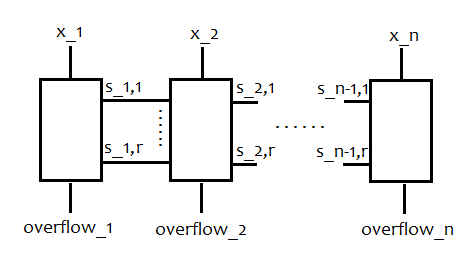
\includegraphics[width=\textwidth]{Sinz_seq.png}
\caption{Sequentieller Counter von Sinz in Anlehnung an \cite[][] {sinz}}
\label{fig:sinz_counter}
\end{figure}

Jeder Addierer erhält eine Eingangsvariable und $r$-viele Teilsummen als Eingänge. Es gibt $n$ Addierer und bei jedem geht ein Overflow-Bit heraus. Die entstehenden Überträge der einzelnen Addierer werden auf true gesetzt, wenn die Teilsumme größer als $r$ ist. Damit die Cardinality Constraints erfüllbar sein können, sind keine Überträge erlaubt, somit werden sie auf false gesetzt. Diese Aufgabe übernimmt der Comparator. Es wird ausgenutzt, dass $\neg \text{overflow}_i$ für $1 \leq i \leq n$ gelten muss, um den Schaltkreis zu vereinfachen. Daraus ergeben sich dann eine Menge von Klauseln.

Bei dieser Variante werden erneut anhand von \cite[][]{knuth} neue Variablen eingeführt. Es werden $(n-r)*r$ neue Variablen der Form $\text{s}_j^k$ für $1 \leq j \leq n - r$ und $1 \leq k \leq r$ gebildet. \\
Mit den neuen Variablen können folgende Klauseln erstellt werden:\\
\textbf{1. Formel:}\\
$(\neg \text{s}_j^k \vee \text{s}_{j+1}^k)$ für $(1 \leq j \textless n - r)$ und $(1 \leq k \leq r)$\\
\textbf{2. Formel:}\\
$(\neg \text{x}_{j+k} \vee \neg \text{s}_j^k \vee \text{s}_j^{k+1})$ für $1 \leq j \leq n - r$ und $0 \leq k \leq r$\\

Die Variablen der Form  $\neg s_j^0$ können gestrichen werden. Dies ist möglich, weil sie nur in der negierten Form vorkommen. Des Weiteren dürfen Variablen der Form $\text{s}_j^{r+1}$ gestrichen werden, weil sie nur positiv vorkommen.

	\subsubsection{Beispiel für eine sequentielle Kodierung}
Es ergeben sich für das Beispiel von $n=4$ und $r=1$ folgende Variablen:\\
\textbf{Formel 1:}\\
Da $1 \leq j \textless 3$ ergeben sich $1$ oder $2$ für j.\\
Für $k$ ergibt sich $1$, da $1 \leq k \leq 1$.\\
$\neg \text{b}_1^1 \vee \text{b}_2^1$\\
$\neg  \text{b}_2^1 \vee \text{b}_3^1$\\
In diesem Fall können keine Variablen gestrichen werden.\\

\textbf{Formel 2:}\\
Bei dieser Formel kann j $1, 2$ oder $3$ sein, da $1 \leq j \leq 3$ . Die Variable $k$ kann $0$ oder $1$ sein, da $0 \leq k \leq 1$.\\
\textbf{k = 0:}\\
$\neg x_1 \vee \neg b_1^0 \vee b_1^1$\\
$\neg x_2 \vee \neg b_2^0 \vee b_2^1$\\
$\neg x_3 \vee \neg b_3^0 \vee b_3^1$\\
\textbf{k =1:}\\
$\neg x_2 \vee \neg b_1^1 \vee b_1^2$\\
$\neg x_3 \vee \neg b_2^1 \vee b_2^2$\\
$\neg x_4 \vee \neg b_3^1 \vee b_3^2$\\

Alle trivialen Variablen werden gestrichen. Diese Klauseln bleiben bestehen:\\
\textbf{k = 0:}\\
$\neg x_1 \vee b_1^1$\\
$\neg x_2 \vee b_2^1$\\
$\neg x_3 \vee b_3^1$\\
\textbf{k =1:}\\
$\neg x_2 \vee \neg b_1^1 $\\
$\neg x_3 \vee \neg b_2^1 $\\
$\neg x_4 \vee \neg b_3^1 $\\

Die vollständige KNF sieht folgendermaßen aus:\\
$(\neg b_1^1 \vee b_2^1) \wedge (\neg b_2^1 \vee b_3^1) \wedge (\neg x_1 \vee b_1^1) \wedge (\neg x_2 \vee b_2^1) \wedge (\neg x_3 \vee b_3^1) \wedge (\neg x_2 \vee \neg b_1^1) \wedge (\neg x_3 \vee \neg b_2^1) \wedge (\neg x_4 \vee \neg b_3^1) $\\

		\subsubsection{parallel}
Der Unterschied zum sequentiellen Counter besteht darin, dass beim parallelen Counter die Eingangsvariablen in zwei Hälften geteilt werden und durch Sub-Counter parallel verarbeitet werden können. Die erste Hälfte hat die Größe $2^m$ mit  $2^m \leq n \textless 2^{m+1}, m \in \mathtt{N}$. Damit die zweite Hälfte nie weniger Eingangsvariablen enthält als die erste, gibt es den Sonderfall, dass die zweite Hälfte keine Eingangsvariablen hat. Gibt es nur eine Eingangsvariable wird diese direkt in den Output weiter geleitet.\\
Im nächsten Schritt wird rekursiv in den Countern berechnet wie groß die Anzahl der Eingangsvariablen ist, die auf true gesetzt werden müssen. Die Ausgangsvariable des ersten Counters wird mit der entsprechenden Ausgangsvariable des zweiten Counters durch einen Volladdierer zusammen gerechnet. Falls der zweite Counter weniger Ausgangsvariablen hat als der erste werden nur Halbaddierer benötigt. Die letzte Eingangsvariable wird als Carry-Bit in den letzten Addierer gegeben. Die Counter berechnen somit parallel die Summe von $2^m-1$ Eingangsvariablen.\\

\begin{figure}[H]
\centering
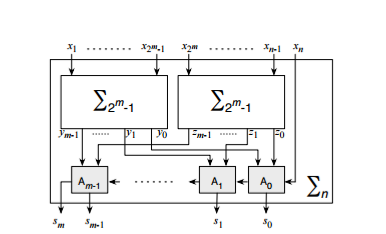
\includegraphics[width=9cm]{Sinz_para.png}
\caption{Paralleler Counter von Sinz \cite[siehe][Seite 9] {sinz}}
\label{fig:sinz_counter_para}
\end{figure}

Es wird ausgenutzt, dass Volladdierer drei Inputs, aber nur zwei Outputs haben. Dadurch können Leitungen reduziert werden. Des Weiteren kann durch die Anzahl der Eingangsvariablen ($n$) und den $m+1$ Outputs gesagt werden, dass der Schaltkreis aus $n-(m+1)$ Volladdierern besteht. Die Anzah der Halbaddierer ist kleiner oder gleich $m$.\\

Der Halb-Addierer und Voll-Addierer kann folgendermaßen als KNF ausgedrückt werden:\\
Der Halb-Addierer besteht aus drei Klauseln:
\begin{itemize}
\item $(a \vee \neg carryIn \vee sum)$
\item $(\neg a \vee carryIn \vee sum)$
\item $(\neg a \vee \neg caaryIn \vee carryOut )$
\end{itemize}

Der Voll-Addierer besteht aus sieben Klauseln:
\begin{itemize}
\item $(a \vee b \vee \neg carryIn \vee sum)$
\item $( a \vee \neg b \vee carryIn \vee sum)$
\item $(\neg a \vee b \vee caaryIn \vee sum )$
\item $(\neg a \vee \neg b \vee \neg carryIn \vee sum)$
\item$(\neg a \vee \neg b \vee carryOut)$
\item$(\neg a \vee \neg carryIn \vee carryOut)$
\item$(\neg b \vee carryIn \vee carryOut)$
\end{itemize}

Zum Schluss wird noch ein Comparator benötigt, damit die Summe mit $r$ verglichen werden kann. Es werden rekrusiv die Klauseln für den Comparator generiert.
\begin{align*}
&L(k_0) = \begin{cases} \{\{\neg s_0\}\} & if{~}k_0 = 0\\ \emptyset & if{~}k_0=1\end{cases}\\
&L(k_i \dots k_0) = \begin{cases} \{\{\neg s_i\}\}\cup L(k_{i-1} \dots k_0) & if{~}k_i = 0\\  \{\{\neg s_i\}\}\otimes L(k_{i-1} \dots k_0) & if{~}k_i = 1\end{cases}
\end{align*}

Als Erstes werden die Klauseln mit $\otimes$ aufgeteilt und $L(k_{m} \dots k_0)$ ist die Menge an Klauseln, die sicher stellt, dass der Output des Counters kleiner oder gleich $r$ ist. Für jede $0$ in der binären Repräsentation wird eine neue Klausel generiert.
Die Repräsentation von $r$ ist binär, so dass die Belegung der Outputs mit der binären Repräsentation von $r$ verglichen werden kann.

\subsubsection{Beispiel für eine parallele Kodierung}
Für dieses Beispiel wird $n=9$ gesetzt, so dass $2^3 \leq 9 \textless 2^4$ ist. Somit ergibt sich für dieses Beispiel, dass es Volladdierer und Halbaddierer gibt. Der Aufbau der Schaltkreise wird in den folgenden Abbildungen dargestellt.

\begin{figure}[H]
\centering
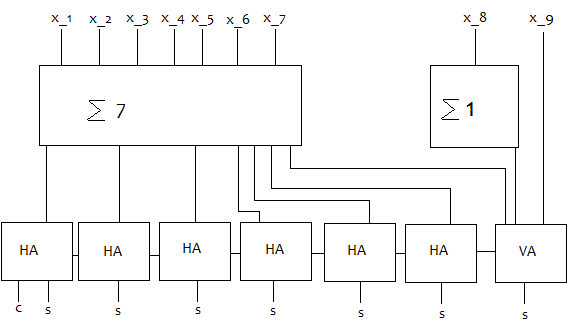
\includegraphics[width=\textwidth]{Bsp_Sinz_grob.png}
\caption{Paralleler Counter von Sinz für $n=9$}
\label{fig:sinz_counter_para_bsp}
\end{figure}

Durch die hohe Summe für die erste Hälfte der Eingangsvariablen ($\sum7$) wird der Schaltkreis weiter unterteilt dargestellt.

\begin{figure}[H]
\centering
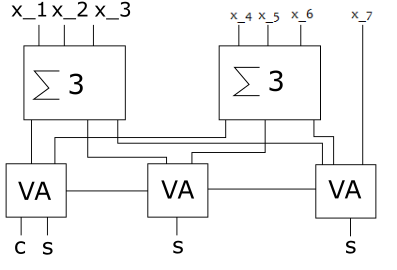
\includegraphics[width=\textwidth]{Bsp_Sinz_fein.png}
\caption{Paralleler Counter von Sinz für $n=7$}
\label{fig:sinz_counter_para_bsp}
\end{figure}

Das Beispiel besteht aus $11$ Volladdierern sowie 6 Halbaddierern und aus $95$ Klauseln für den Schaltkreis.\\

\textbf{Beispiel für den Comparator anhand von $r$}:\\
Sei $r = 18$, in binärer Repräsenation ist dies $10010$. Daraus ergeben sich 3 Klauseln, da es drei Nullen gibt und 5 verschiedene Variablen, bei denen die Variablen mit einer $0$ nur negiert aufgeschrieben werden. Das bedeutet, dass $x_0 = \bot, x_1 = \top, x_2 = \bot, x_3 = \bot, x_4 = \top$.\\
Die folgenden Klauseln können gebildet werden:\\
\begin{itemize}
\item $\{\neg x_0\}$ (Variale wird nur negiert aufgeschrieben)
\item  $\{\neg x_0,\neg x_1\}$ (Variable wird in alle bestehenden Mengen hinzugefügt)
\item $\{\{\neg x_0, \neg x_1\},\{\neg x_2\}\}$
\item $\{\{\neg x_0, \neg x_1\},\{\neg x_2\}, \{\neg x_3\}\}$
\item $\{\{\neg x_0, \neg x_1\, \neg x_4\},\{\neg x_2, \neg x_4\}, \{\neg x_3, \neg x_4\}\}$
\end{itemize}


	\subsection{Kodierung basierend auf BDDs}
Mit Hilfe von BDDs können Cardinality Constraints in Klauseln übersetzt werden. Dafür werden die Constraints in den BDDs dargestellt und aus dem BDD können die Klauseln erstellt werden. Der BDD kann einfach als ein Schaltkreis von if-then-else Gattern angesehen werden, der durch die Tseitin Transformation zu Klauseln übersetzt wird. Der Algorithmus aus \cite[][Seite 11]{niklasse} musste angepasst werden, da er nur für $\geq$ Constraints funktioniert und nicht für $\leq$ Constraints. Dafür wurde für die Koeffizienten  immer eine $1$ eingesetzt, da es dem in dieser Arbeit dbetrachteten Falll keine Koeffizienten gibt, bzw. der Koeffizient immer $1$ ist. Beim Erstellen der ITE-Gates wurden hi\_result und lo\_result vertauscht.\\

\begin{algorithm}
\caption{buildBDD (vec<int> Cs, vec<signal> ps, int rhs, int size, int sum, int material\_left, map<pai<int,int>, signal> memo)}
\label{alg:buildBDD}
\begin{algorithmic}

\State $\text{}if (sum \leq rhs)$
\State $\text{~~return } TRUE$
\State $\text{}else if (sum + material\_left \textless rhs)$
\State $\text{~~return } FALSE$
\State $\text{} key = (size, sum)$
\State $\text{}if (memo[key] == UNDEF) \{$
\State $\text{~~} size\text{-{}-}$
\State $\text{~~} material\_left \text{-{}-}$
\State $\text{~~} hi\_sum = sign(ps[size]) ? sum : sum + 1$
\State $\text{~~} hi\_sum = sign(ps[size]) ? sum + 1 : sum$
\State $\text{~~} hi\_result = buildBDD(ps , rhs, size, hi\_sum, material\_left, memo)$
\State $\text{~~} lo\_result = buildBDD(ps , rhs, size, lo\_sum, material\_left, memo)$
\State $\text{~~} memo[key] = ITE(var(ps[size]), lo\_result, hi\_result)\}$
\State $\text{return }memo[key]$
\end{algorithmic}
\end{algorithm}

Beim Aufruf der Methode wird size auf die Anzah der Koeffizienten auf der linken Seite des Constraints gesetzt, sum auf $0$, material\_left ist die Summe aller Koeffizienten auf der linken Seite und memo ist eine leere Map. Für die weiteren Befehle ist sign(p) true oder false der Literale und var(p) gibt die zugrunde liegende Variable des Literals zurück.\\

Der Algorithmus konstruiert den BDD, indem die Variablen nacheinander abgearbeitet werden. Dann wird das ITE-Gate erstellt mit dem Literal als Knotenbeschriftung und einer low- und high-Kante unterhalb des Knotens. Durch das Hinzunehmen der Tseitin-Variablen, kann der key herausgefunden werden und damit welcher Knoten zu welchem Eltern-Knoten gehört.\\
Eine weitere Aufgabe bestand darin, dass die ITE-Gates mit Tseitin als Konjunktive Normalform repräsentiert werden müssen (t ist dabei die Tseitin-Variable und a,b und c die unterschiedlichen Inputs). Dies kann folgendermaßen hergeleitet werden:\\
\begin{align*}
\begin{aligned}
&t \leftrightarrow ite(a,b,c)\\
&(t \rightarrow ite (a,b,c)) \wedge (ite (a,b,c) \rightarrow t)\\
&(\neg t \vee ite(a,b,c)) \wedge (\neg ite(a,b,c) \vee t)\\
&(\neg t \vee (a \wedge b) \vee (\neg a \wedge c)) \wedge (\neg((a \wedge b) \vee (\neg a \wedge c)) \vee t)\\
&(\neg t \vee (a \wedge b) \vee (\neg a \wedge c)) \wedge ((\neg(a \wedge b) \wedge \neg (\neg a \wedge c)) \vee t\\
&(\neg t \vee (a \wedge b) \vee (\neg a \wedge c)) \wedge ((\neg a \vee \neg b) \wedge (a \vee \neg c)) \vee t\\
&(\neg t \vee (a \wedge b) \vee (\neg a \wedge c)) \wedge (\neg a \vee \neg b \vee t) \wedge (a \vee \neg c \vee t)\\
&(\neg t \vee a \vee \neg a) \wedge (\neg t \vee a\vee c) \wedge (\neg t \vee b \vee \neg a) \wedge (\neg t \vee b \vee c) \wedge (\neg a \vee \neg b \vee t) \wedge (a \vee \neg c \vee t)\\
&\neg t \vee a\vee c) \wedge (\neg t \vee b \vee \neg a) \wedge (\neg a \vee \neg b \vee t) \wedge (a \vee \neg c \vee t)
\end{aligned}
\end{align*}

%Ein ITE-Gate sagt nichts anderes als if (a then b else c) und das bedeutet $(a \wedge b) \vee (\neg a \wedge c)$. Daher kann dies in Schritt 4 eingesetzt werden. Die Klausel $(\neg t \vee a \vee \neg a)$ kann entfernt werden, da $(a \vee \neg a)$ immer $1$ ist und somit die ganze Klausel $1$ ist. Die Klausel $(\neg t \vee b \vee c)$ wird aus Performanzgründen nicht verwendet. Dies ist erlaubt, da durch sie eine Resolvente der Klauseln ...

	\subsection{naive Kodierung basierend auf Sorting Networks}
Sorting Networks stellen einen effektiven Weg dar, um Cardinality Constraints zu implementieren. Nachdem die Eingangsvariablen durch das Sorting Network sortiert wurden, kann schnell abgelesen werden, ob das Constraint erfüllt werden kann oder nicht.
Beim Constraint $\leq r$ dürfen nicht mehr als $r$ Ausgänge mit true belegt sein. Sind mehr als $r$ Ausgänge mit true belegt, kann der SAT-Solver schnell feststellen, dass dieses Cardinality Constraint nicht erfüllbar ist.\\
Die Comparators können durch verschiedene Algorithmen angeordnet werden. Für die naive Variante wird der Bubble-Sort-Algorithmus verwendet. Der Aufbau des Netzes lässt sich folgendermaßen darstellen:\\

\begin{figure}[H]
\centering
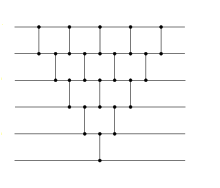
\includegraphics[width=9cm]{sorting_network_bubble.png}
\caption{Sorting Network mit Bubble-Sort}
\label{fig:sorting_network_naiv_bsp}
\end{figure}

In Abbilung \ref{fig:sorting_network_naiv_bsp} gibt es die Eigangsvariablen $x_0$ bis $x_5$, daher ist $n=6$. Jedes Mal wenn an einem Comparator am oberen Eingang false und am unteren Eingang true anliegen, wird getauscht (siehe Abbilung \ref{fig:sorting_network_naiv_bsp1}).

\begin{figure}[H]
\centering
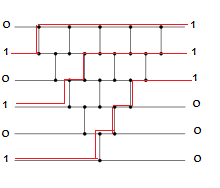
\includegraphics[width=9cm]{sorting_network_bubble_rot.png}
\caption{Sorting Network mit Bubble-Sort und markierten Leitungen}
\label{fig:sorting_network_naiv_bsp1}
\end{figure}

Die folgende KNF beschreibt das Verhalten eines einzelnen Comparators:\\
$(\neg output_2 \vee output_1) \wedge (\neg input_1 \vee \neg input_2 \vee output_2) \wedge (input_1 \vee \neg output_2) \wedge (input_2 \vee \neg output_2) \wedge (input_1 \vee input_2 \vee \neg output_1) \wedge (\neg input_1 \vee output_1) \wedge (\neg input_2 \vee output_1)$

	\subsection{Sorting Networks mit Odd-Even Mergesort}
Als Grundlage für die eigene entwickelte Kodierung dient das Sorting Network mit einem Odd-Even Mergesort. Der Unterschied zur naiven Kodierung ist der, dass nicht der Bubblesort als Sortieralgorithmus verwendet wird, sondern der Odd-Even Mergesort. Dadurch entsteht ein Netz mit anders angeordneten Comparators.

\begin{figure}[H]
\centering
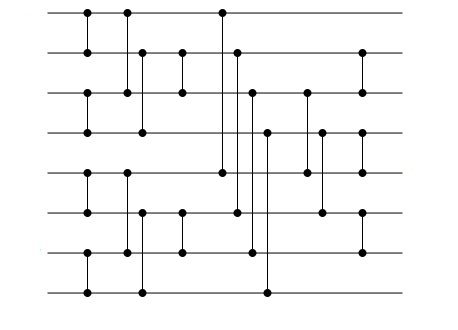
\includegraphics[width=\textwidth]{odd-even-mergesort.png}
\caption{Sorting Network mit Odd-Even-Mergesort}
\label{fig:odd-even-mergesort}
\end{figure}

Durch die andere Anordnung der Comparators durch den Odd-Even Mergesort können Comparators eingespart werden, was zu einer Performanzsteigerung führt. Beim Odd-Even Mergesort werden die Eingänge in zwei Hälften geteilt und zunächst rekursiv sortiert. Im Anschluss daran werden die beiden sortierten Hälften wieder zusammengeführt. Beim Mergen werden immer die benachbarten Elemente verglichen.\\
Normalerweise ist $n$ immer eine Potenz von $2$ beim Odd-Even-Mergesort. Dies ist nicht immer möglich, daher wird bei anderen Werten auf die entsprechende Zweierpotenz aufgerundet. Das Sorting-Network wird rekursiv aufgebaut und entsprechend vergrößert. In Abbildung \ref{fig:odd-even-mergesort} sieht man das Sorting-Network für $n=8$. Die erste Hälfte besteht aus zwei $4$-Input Merge-Sorters. Das selbe gilt auch für die zweite Hälfte. Nachdem die einzelnen Hälften sortiert sind, werden die beiden Hälften ab dem dritten Comparator bei der ersten Leitung gemergt. Das Ergebnis ist dann eine korrekt sortierte Folge.

%TODO eigenen Namen für die Kodierung
	\subsection{Eigene entwickelte Kodierung mit Sorting Networks}
Das Ziel der eigenen Idee für Sorting Networks ist es Comparators zu sparen. Daher wird als Ausgangslage der Odd-Even-Mergesort gewählt, der schon eine reduzierte Anzahl an Comparators hat. Bei der Anwendung von Cardinality Constraints ist immer nur ein einziger Output des Sorting Networks relevant. Daher sind auch nur diejenigen Comparators von Bedeutung, die einen Einfluss auf den Wert des Outputs haben.\\
Nachdem das Odd-Even-Mergesort Network aufgebaut ist, werden diejenigen Comparators entfernt, die nicht im Cone of Influence des $(r+1)$-ten Outputs liegen. Dafür wird das gesamte Network durchsucht. Alle Comparators, deren Outputs
\begin{itemize}
\item nicht mit dem relevanten Output übereinstimmen und
\item nicht als Inputs für noch nicht gestrichene Comparators dienen
\end{itemize}
werden gestrichen. 


%Zur Ideenfindung wurde das Sorting Network aufgemalt und überlegt, wie die entsprechende Leitung von $r$ Einfluss auf die Comparator haben kann. Wird $r=2$ gewählt, so entscheidet der Ausgang an der zweiten Stelle des Sorting Networks, ob eine Belegung gefunden werden kann für das Constraint oder nicht. Liegt an der zweiten Stelle eine $0$ an, dann ist es SAT. Ansonsten ist es UNSAT. Somit ist nur dieser Ausgang von Bedeutung für den SAT-Solver. Daher müssen alle anderen Ausgänge nicht entsprechend sortiert sein. Aus diesem Grund können alle Comparator eingespart werden, die nichts mit der entsprechenden Leitung zu tun haben und auch alle, bei denen die Ein- und Ausgänge der andern Comparator keinen Einfluss auf die Sortierug des zweiten Ausgangs des Sorting Networks haben. Dafür wird das Sorting Network erst einmal aufgebaut wie beim odd-even Mergesort und anschließend wird das gesamte Network mehrmals durchsucht nach Comparator, die gestrichen werden können. Dies muss mehrmals passieren, da erst im Laufe der Zeit herausgefunden werden kann, welche gelöscht werden können. Daraus ergibt sich ein Aufwand von $O(n^3)$.

\subsubsection{Beispiel für die eigene Kodierung}
In der folgenden Abbildung wird das Odd-Even Mergesort Network dargestellt und daran wird das Entfernen der Comparators beschrieben. Hierbei ist $r=8$, daher ist der letzte Ausgang vom Sorting Network entscheidend.

\begin{figure}[H]
\centering
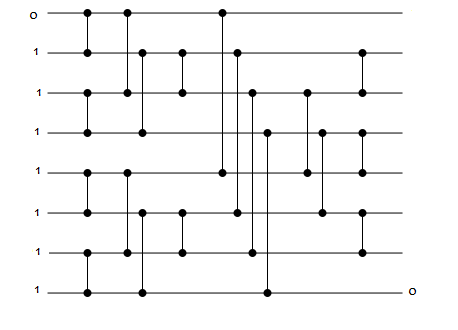
\includegraphics[width=\textwidth]{ownSorting_start.png}
\caption{Ausgangssituation der eigenen Kodierung}
\label{fig:ownSorting}
\end{figure}

Da die Liste der Comparators rückwärts durchlaufen wird, können nacheinander die entsprechenden Comparators entfernt werden. Abbildung \ref{fig:ownSorting1} stellt das fertige Sorting Network dar. Es werden alle Comparators entfernt, die nun keinen Einfluss mehr auf den Ausgang haben. Durch das Wegfallen der letzten drei können die nächsten beiden ebenfalls entfernt werden, da sie für das Ende nichts mehr vorsortieren müssen. Das betrifft auch alle anderen Comparator, die zusätzlich gestrichen werden. 

\begin{figure}[H]
\centering
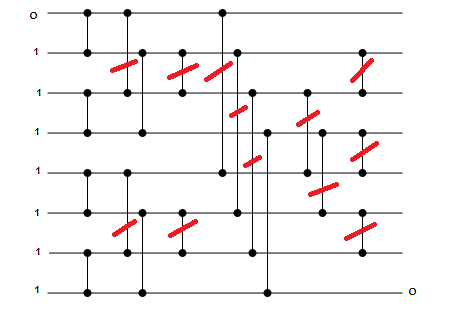
\includegraphics[width=\textwidth]{ownSorting_2.png}
\caption{Entfernen der entsprechenden Comparators}
\label{fig:ownSorting1}
\end{figure}

\begin{figure}[H]
\centering
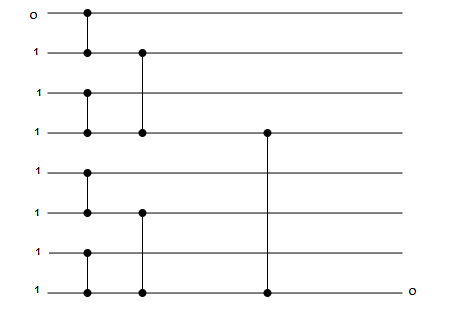
\includegraphics[width=\textwidth]{ownSorting_end.png}
\caption{Fertigiges Sorting Network mit reduzierten Comparators}
\label{fig:ownSortingEnd}
\end{figure}


\section{Umsetzung}
 Als Testproblem für die unterschiedlichen Kodierungen wird das n-Damen-Problem verwendet, da dieses Problem eine wichtige Rolle in der Informatik spielt und viele Constraints abgeleitet werden können. In jeder Reihe (vertikal, horizontal und diagonal) ist nur eine Dame erlaubt. Somit ergeben sich unterschiedliche Kombinationen, die für die Belegung der Literale nur erlaubt sind. Ziel ist es eine Belegung zu finden, die alle Bedingungen erfüllt. 

\begin{figure}[H]
\centering
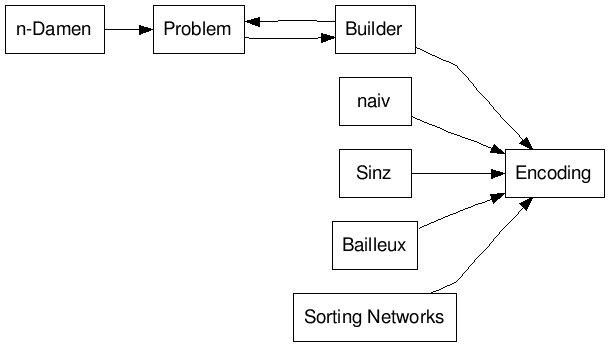
\includegraphics[width=\textwidth]{architektur.png}
\caption{Die Architektur der Implementierung}
\label{fig:architektur}
\end{figure}

In Abbildung \ref{fig:architektur} ist dargestellt, wie die grundlegende Architektur aufgebaut ist. 
Der Builder ist die Zwischenschicht zwischen den Problemen und den unterschiedlichen Kodierungen. Er erstellt das Encoding und ermöglicht dadurch den Aufruf verschiedener Kodierungen. In dieser Klasse werden die verschiedenen Constraints für $\leq$, 	$\geq$ und $\doteq$ gebaut und der Solver wird aufgerufen. Die Klasse Encoding dient als Oberklasse und ist abstrakt, damit die Signatur für die Unterklassen (Kodierungen) vorgegeben ist. 

\section{Evaluation}

\section{Schlussfolgerung und Ausblick}

%Sogar zitieren kann man \textbackslash o/ \cite[vgl.][]{invincible}.


%\begin{algorithm}
%\caption{Minimax-Suche}
%\label{alg:minimax}
%\begin{algorithmic}
%\State $\text{minimax(Spielstellung s)}$
%\State $\text{~~~~falls }spielende(s)$
%\State $\text{~~~~~~~~return }payoff(s)$
%\State $\text{~~~~} v \gets -\infty$
%\State $\text{~~~~für alle möglichen Züge }m$
%\State $\text{~~~~~~~~} f"uhreZugAus(s, m)$
%\State $\text{~~~~~~~~} v' \gets -minimax(s)$
%\State $\text{~~~~~~~~} nimmZugZur"uck(s, m)$
%\State $\text{~~~~~~~~falls }v' > v$
%\State $\text{~~~~~~~~~~~~}v \gets v'$
%\State $\text{~~~~return } v$
%\end{algorithmic}
%\end{algorithm}

%\begin{table}
%\centering
%\small %macht die Schrift kleiner
%\setlength{\tabcolsep}{.11cm} %macht den seitlichen Rand der Zellen kleiner (und damit die Tabelle schmaler)
%\begin{tabular}{|c||c|c|c|C{1.3cm}|c||c|}
%\hline
% & Base & Setup & Heuristics & Chance Pruning & Extensions & Gesamt \\ \hline \hline
%Base & - & $20$ & $22$ & $16,5$ & $18,5$ & $77$\\ \hline
%Setup & $30$ & - & $23,5$ & $19,5$ & $23$ & $96$\\ \hline
%Heuristics & $28$ & $26,5$ & - & $19,5$ & $23,5$ & $97,5$ \\ \hline
%ChancePruning & $33,5$ & $30,5$ & $30,5$ & - & $27$ & $121,5$\\ \hline
%Extensions & $31,5$ & $27$ & $26,5$ & $23$ & - & $108$ \\ \hline
%\end{tabular}
%\caption{Paarweise Ergebnisse des Turniers}
%\label{tab:roundrobin}
%\end{table}

	\clearpage
	\appendix
	\section{Literaturverzeichnis}
		% Latex-Magie von http://tex.stackexchange.com/questions/22645/hiding-the-title-of-the-bibliography
		\begingroup
			\renewcommand{\section}[2]{}
			\bibliographystyle{natdin}
			\bibliography{referenzen}
		\endgroup
\clearpage
	\section{Abbildungsverzeichnis}
		\begingroup
			\renewcommand{\section}[2]{}
			\listoffigures
		\endgroup
	\section{Tabellenverzeichnis}
		\begingroup
			\renewcommand{\section}[2]{}
			\listoftables
		\endgroup
\end{document}
